\chapter{Exploring Parameter Importance}
\label{ch:parameter_importance}

\section{Overview}

Before attempting to optimize FINUFFT's parameters, it is necessary to understand which parameters actually matter and to what degree. This chapter presents a global sensitivity analysis of FINUFFT's configuration space.  We first identify where transform time is actually spent across the three transform types (Section~\ref{sec:stage_breakdown}), then use a global, Gaussian process based search to rank the tunable parameters by their contribution to performance (Section~\ref{sec:gp_sensitivity}). The resulting ranking motivates the choice of parameters treated in depth in Chapters~\ref{ch:sigma_selection} and~\ref{ch:parameter_tuning}.

\section{FINUFFT's Configuration Parameters}

FINUFFT exposes its tunable behaviour through a single options structure called \texttt{finufft\_opts}. Its fields fall into three groups. Data handling options (\texttt{modeord}, \texttt{spreadinterponly}) change the convention used to order output modes or restrict the call to spreading/interpolation only, and do not by themselves change the amount of work performed. Diagnostic options (\texttt{debug}, \texttt{spread\_debug}, \texttt{showwarn}) control logging and are irrelevant to performance. The remaining, performance relevant options are:
\begin{itemize}
    \item \texttt{nthreads}: number of threads used for the transform.
    \item \texttt{spread\_sort}: whether nonuniform points are sorted before spreading (\texttt{0} off, \texttt{1} on, \texttt{2} heuristic choice).
    \item \texttt{upsampfac}: the upsampling factor $\sigma$ real number in the range $[1.25;2.00]$, treated in depth in Chapter~\ref{ch:sigma_selection}.
    \item \texttt{spread\_thread} and \texttt{maxbatchsize}: control how work is split across threads when multiple strength vectors share the same nonuniform points (vectorized calls, $n_{\mathrm{tr}} > 1$).
    \item \texttt{spread\_nthr\_atomic}: thread count above which the spreader switches from an OpenMP critical section to atomic updates.
    \item \texttt{spread\_max\_sp\_size} ($S_{\max}$): integer in the range $[1;\frac{M}{nthr}]$, the maximum number of points in a subproblem of the spreader, written $S_{\max}$ in the rest of this thesis, treated in depth in Chapter~\ref{ch:parameter_tuning}.
    \item the sort bin dimensions $b_x$, $b_y$ and $b_z$: integers in the range $[1;N_d]$ the size in fine-grid cells of the boxes the nonuniform points are binned into before spreading. Unlike the other entries in this list they are not fields of \texttt{finufft\_opts} at all but constants in the source, fixed at $16$ along the fast axis and $4$ along the slower ones; they are exposed as options here in order to include them in the search, and are treated in depth in Chapter~\ref{ch:parameter_tuning}.
\end{itemize}
Two further fields, \texttt{spread\_kerevalmeth} and \texttt{spread\_kerpad}, are retained only for binary compatibility and have no effect on current versions of the library. A third, \texttt{spread\_kerformula}, is reserved for internal debugging. All three are therefore excluded from the analysis that follows.

\section{Where Does Time Go? Stage-Level Breakdown}
\label{sec:stage_breakdown}

Every FINUFFT call proceeds through three stages, introduced in Chapter~\ref{ch:background}: \texttt{makeplan}, which precomputes kernel coefficients and creates the FFT plan; \texttt{setpts}, which sorts and preprocesses the nonuniform points; and \texttt{execute}, which performs the actual spreading, FFT, and deconvolution. Before deciding which configuration parameters deserve attention, it is useful to know how much of the total runtime each stage typically accounts for, since a parameter that only affects a negligible stage cannot meaningfully improve overall performance.

Using the benchmark configurations distributed with FINUFFT (covering a range of precisions, tolerances, dimensions, and both extremal values of $\sigma$), each call was timed and the three stage durations were normalised so that they summed to one. Figure~\ref{fig:stage_breakdown} shows the resulting distribution, split by transform type. For type 1 and type 2 transforms, \texttt{execute} dominates, accounting for the large majority of the total time, while \texttt{setpts} contributes a smaller but non-negligible share and \texttt{makeplan} is close to zero in almost every case. Type 3 transforms show a markedly different balance: \texttt{setpts} and \texttt{execute} contribute comparable shares, reflecting the additional preprocessing type 3 transforms require to handle nonuniform points on both sides of the transform.

\begin{figure}[h]
    \centering
    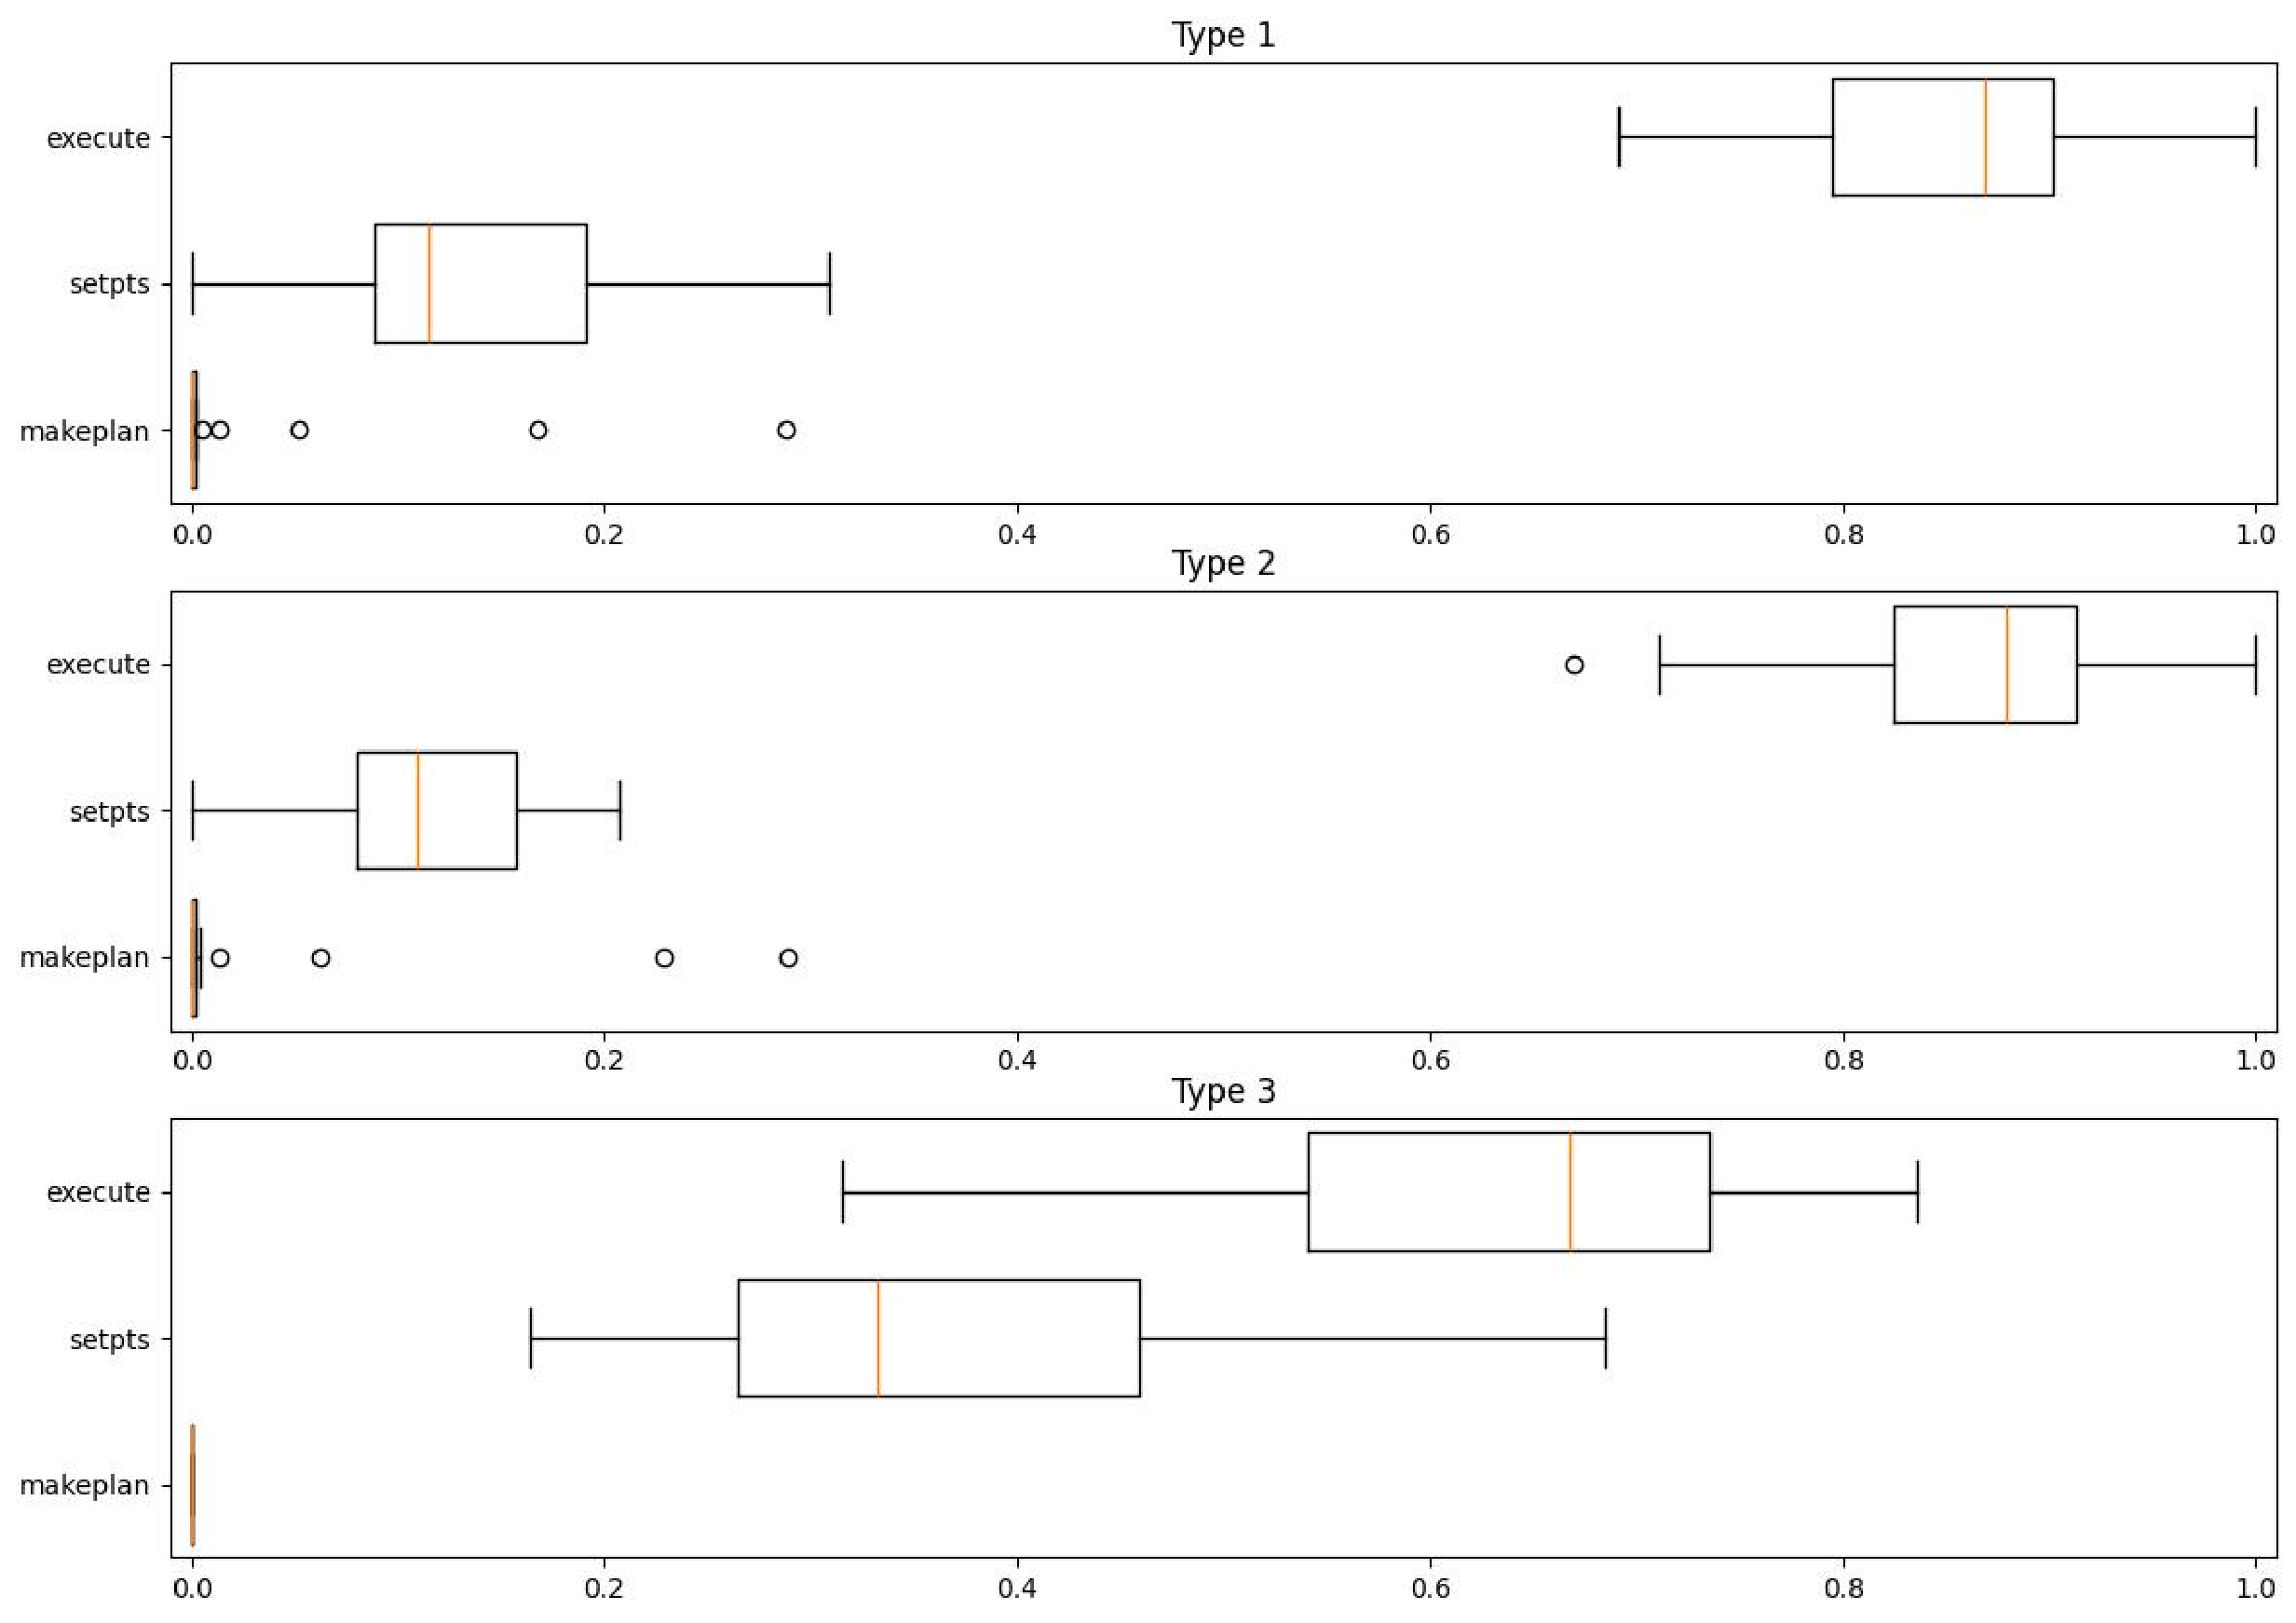
\includegraphics[width=0.85\textwidth]{figures/parameter_importance/stage_breakdown.pdf}
    \caption{Fraction of total call time spent in each stage (\texttt{makeplan}, \texttt{setpts}, \texttt{execute}), by transform type.}
    \label{fig:stage_breakdown}
\end{figure}

This picture was refined further by instrumenting \texttt{setpts} itself, splitting it into its constituent substeps: precomputing kernel Horner coefficients, evaluating the kernel Fourier series used for deconvolution, and creating the FFT plan. These substeps behave largely as fixed, per-call overheads rather than costs that scale with the number of nonuniform points $M$, which is consistent with \texttt{makeplan} and the fixed portion of \texttt{setpts} contributing a shrinking fraction of total time as $M$ grows.

Together, these observations indicate that parameters affecting the \texttt{execute} stage, and specifically the spreading and FFT steps within it, offer the largest potential impact on performance, with parameters affecting \texttt{setpts} becoming relevant mainly for type 3 transforms or when $M$ is small enough that fixed overheads are not amortised.

\section{Global Sensitivity Analysis via Gaussian-Process Optimization}
\label{sec:gp_sensitivity}

Stage-level timing shows which stage costs time, but not which of the many configuration parameters within that stage is responsible, nor how the parameters interact. To rank the parameters directly, a Gaussian process based Bayesian optimizer~\cite{rasmussen2006,snoek2012} (as implemented in Optuna~\cite{optuna2019}) was used to search the joint space of \texttt{spread\_max\_sp\_size} ($S_{\max}$), \texttt{spread\_sort}, \texttt{upsampfac}, \texttt{spread\_nthr\_atomic} and the two sort bin dimensions $b_x$ and $b_y$, minimising the measured time of \texttt{setpts} plus \texttt{execute} for a single type 1 transform whose nonuniform point data occupies one gibibyte (two dimensions, double precision, $M = 2^{30}/32 = 33{,}554{,}432$ points on a $5793 \times 5793$ grid, so one point per fine-grid cell, $\mathrm{tol} = 10^{-6}$). Every thread of the node was used, $64$ in all. \texttt{setpts} is inside the timed region because the bin sort happens there, and a measurement of \texttt{execute} alone could not see the bin dimensions at all. Two parameters were given ranges rather than the handful of values the library exposes: \texttt{upsampfac} was sampled continuously over $[1.25, 2.00]$, and \texttt{spread\_max\_sp\_size} ($S_{\max}$) was sampled from $10^3$ up to $M/n_{\mathrm{thr}}$. \texttt{spread\_thread} and \texttt{maxbatchsize} were left out of the search, since both only affect vectorized calls ($n_{\mathrm{tr}} > 1$) and this workload uses a single strength vector; \texttt{modeord}, the FFT planner flag and the internal kernel formula selector were likewise excluded, as none is intended to be tuned per call.

In the search, the best configuration found completed the transform in $0.474$\,s, against $0.509$\,s for the library defaults at this tolerance ($\sigma = 1.25$, sorting on, bins $16 \times 4$, \texttt{spread\_max\_sp\_size} ($S_{\max}$) $= 10^5$); these are the two times marked in Figure~\ref{fig:gp_histogram}. A single trial can be favoured by noise, so both configurations were then re-measured five times each on the same node, giving means of $0.4825$\,s and $0.5087$\,s with ranges that do not overlap. The best configuration therefore improves throughput by $0.5087/0.4825 - 1 \approx 5.4\%$, or equivalently reduces the time by $5.4\%$. Table~\ref{tab:gp_best} lists the parameter values that achieved it. The modest margin is itself the result: for a transform of this size and density the defaults are already close to the best these six parameters can do, and what headroom remains lies in the bin dimensions rather than in the subproblem size. Note also that the best configuration agrees with the defaults on $\sigma$ and on sorting, so the $5.4\%$ is attributable entirely to \texttt{spread\_max\_sp\_size} ($S_{\max}$), \texttt{spread\_nthr\_atomic} and the two bin dimensions.

Figure~\ref{fig:gp_histogram} shows the distribution of times across all completed trials on a logarithmic axis, with the default and the best configuration marked. The majority of trials cluster within a factor of a few of the default, and a right tail of badly performing configurations runs past the eight-second cap at which trials were stopped; the best configuration sits at the front edge of the main cluster rather than being an isolated outlier, indicating that a good configuration is common while a specific region of the search space is very bad.

\begin{table}[h]
    \centering
    \begin{tabular}{lll}
        \hline
        \textbf{Parameter} & \textbf{Default} & \textbf{Best value found} \\
        \hline
        \texttt{spread\_max\_sp\_size} ($S_{\max}$) & $10^5$ & 5085 \\
        \texttt{spread\_sort} & 1 (on) & 1 (on) \\
        \texttt{upsampfac} & 1.25 & 1.25 \\
        \texttt{spread\_nthr\_atomic} & atomic update & atomic update \\
        $b_x \times b_y$ & $16 \times 4$ & $24 \times 71$ \\
        \hline
    \end{tabular}
    \caption{Parameter values of the best configuration found by the Gaussian process search, against the values the library uses for this input.}
    \label{tab:gp_best}
\end{table}

\begin{figure}[h]
    \centering
    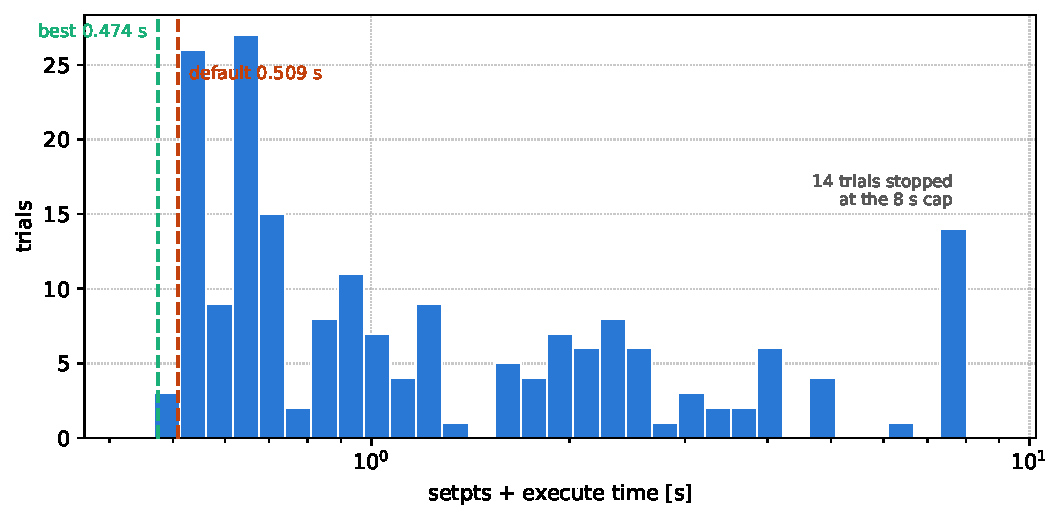
\includegraphics[width=0.8\textwidth]{figures/parameter_importance_2d/optuna_histogram_2d.pdf}
    \caption{Distribution of measured times across the search trials, with the library default and the best configuration found marked; trials slower than the eight-second cap were stopped there rather than measured.}
    \label{fig:gp_histogram}
\end{figure}

To quantify the relative contribution of each parameter, functional ANOVA (fANOVA) importance scores~\cite{hutter2014fanova} were computed from the completed trials. Figure~\ref{fig:importance} shows the result in two panels. Over all trials \texttt{spread\_sort} accounts for $85.7\%$ of the variance in execution time, because leaving the points unsorted at this size costs one to two orders of magnitude and swamps every other effect; \texttt{upsampfac} follows at $10.6\%$ and the remaining four parameters together account for under $4\%$. Conditioning on the trials that sort, which is the regime any sensible configuration is in, ranks the rest against each other: \texttt{upsampfac} dominates at $62.6\%$, the two bin sizes contribute $18.3\%$ and $11.2\%$, \texttt{spread\_nthr\_atomic} $5.4\%$, and \texttt{spread\_max\_sp\_size} ($S_{\max}$) only $2.5\%$. The last of these is a genuine measurement over the whole of that parameter's effective range: the spreader gives every thread one subproblem and only subdivides further when \texttt{spread\_max\_sp\_size} ($S_{\max}$) falls below $M/n_{\mathrm{thr}}$, so values above that bound are indistinguishable from it and the search covered everything below.

\begin{figure}[h]
    \centering
    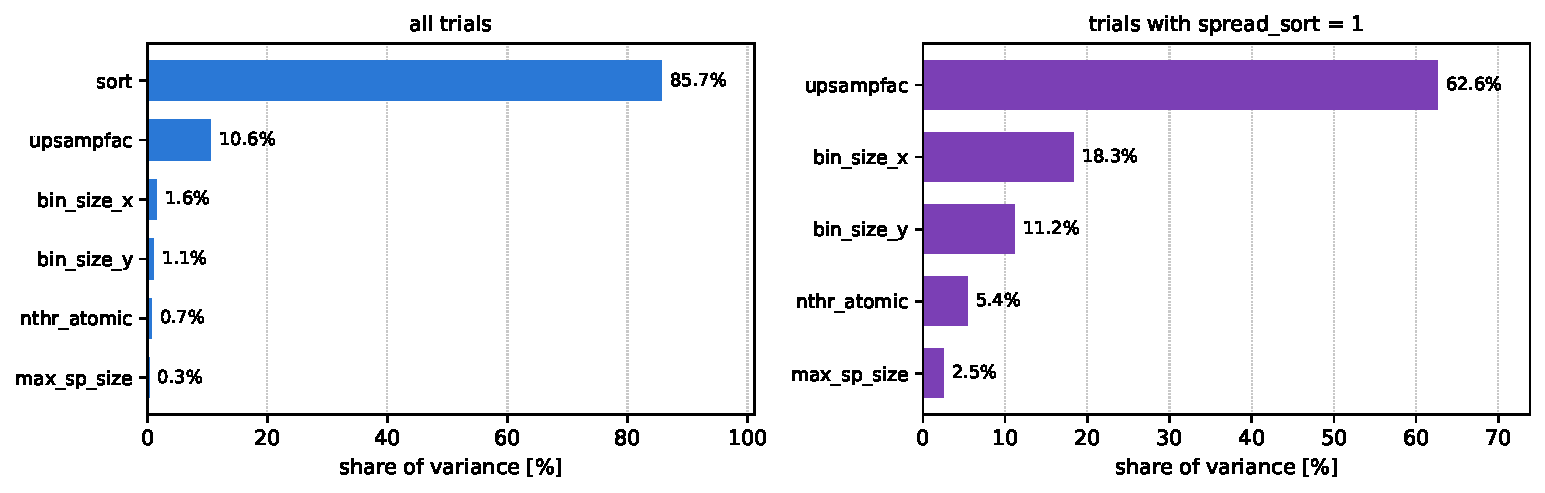
\includegraphics[width=\textwidth]{figures/parameter_importance_2d/importance_2d.pdf}
    \caption{Relative parameter importance from functional ANOVA, over all search trials and over the trials with sorting enabled.}
    \label{fig:importance}
\end{figure}

The dominance of \texttt{spread\_sort} is the least surprising of these results: sorting the nonuniform points by spatial location is what keeps each thread's working set localised, and at this size the unsorted alternative destroys that locality completely. Its share therefore reflects the cost of getting a binary choice wrong rather than headroom the default leaves on the table, since FINUFFT's own heuristic already enables sorting for inputs of this shape. The interesting result is the second panel. \texttt{upsampfac} takes $62.6\%$ of the remaining variance. That it dominates while the best configuration nonetheless agrees with the default value is not a contradiction: $\sigma$ sets the size of the fine grid and hence the whole cost of the FFT, so moving it away from a good value is expensive in a way no amount of spreader tuning can recover, and the score measures that sensitivity rather than any headroom the default leaves. Chapter~\ref{ch:sigma_selection} analyzes it in depth. The two bin dimensions together account for a further $29.5\%$, which Chapter~\ref{ch:parameter_tuning} traces to the cache behaviour of the sort and of the spreading and adding steps downstream of it. \texttt{spread\_max\_sp\_size} ($S_{\max}$), by contrast, contributes only $2.5\%$ here, which is a stronger statement than it appears: the spreader gives each thread one subproblem and subdivides further only when the parameter falls below $M/n_{\mathrm{thr}}$, so values above that bound are indistinguishable from it and the search covered the whole of the range in which the parameter can act at all. That low score measures a share of variance rather than an absence of effect: $\sigma$ sets the size of the whole FFT grid and can multiply the total time several-fold. In absolute terms the subproblem size is far from negligible, and Chapter~\ref{ch:parameter_tuning} shows that it moves the spreading phase of this same transform by a factor of $1.85$, also Chapter~\ref{ch:parameter_tuning} shows that this is not true at every density and thread count, which is why it still merits a dedicated treatment.

\section{Implications for the Remainder of This Thesis}

The stage breakdown and the global sensitivity analysis together justify the choice of parameters examined in the rest of this thesis. \texttt{upsampfac} is the highest-ranked tunable parameter once the binary sorting choice is fixed, and its default is chosen by a heuristic that considers only two values; Chapter~\ref{ch:sigma_selection} analyzes its effects on spreading and FFT steps performance. The sort bin dimensions rank next, and Chapter~\ref{ch:parameter_tuning} examines how they trade the cost of the sort itself against the subgrids it produces. \texttt{spread\_max\_sp\_size} ($S_{\max}$) ranks low for this particular workload, but it governs a nontrivial trade-off between scheduling overhead and load imbalance that becomes severe at other densities and thread counts, so it too receives a dedicated treatment. \texttt{spread\_sort} clearly matters, but its optimal setting is simple, sorting should remain enabled as it already is by default for realistic inputs and \texttt{spread\_nthr\_atomic} contributes little and is not investigated further. \texttt{spread\_thread} and \texttt{maxbatchsize} were excluded from the search itself, since both only affect vectorized multi-transform calls, which fall outside the scope of this thesis.

\section{Summary}

This chapter established where FINUFFT spends its time and which of its configuration parameters have the largest effect on it. Stage-level timing showed that \texttt{execute} dominates type 1 and type 2 transforms, while \texttt{setpts} becomes comparably important for type 3 transforms. A Gaussian process based sensitivity analysis then showed that \texttt{spread\_sort} accounts for most of the variance across the whole search, and that once sorting is fixed on, \texttt{upsampfac} and the sort bin dimensions account for the large majority of what remains, while \texttt{spread\_max\_sp\_size} ($S_{\max}$) accounts for little of the variance on this workload, although its absolute effect on the spreading phase is substantial. The best configuration found ran $5.2\%$ faster than the library defaults. These findings motivate the analyses that follow: an analysis of $\sigma$ and how it trades kernel width against fine-grid size (Chapter~\ref{ch:sigma_selection}), and an analysis of the spreader parameters that govern subproblem and bin geometry (Chapter~\ref{ch:parameter_tuning}).
